\documentclass[twocolumn,10pt]{jarticle}
\setlength{\columnsep}{3zw}
\usepackage{color}
\usepackage[dvipdfmx]{graphicx}
\usepackage{amsmath,amssymb}
\usepackage[linesnumbered,ruled,vlined]{algorithm2e}
\usepackage{bm}
\usepackage[top=10truemm,bottom=20truemm,left=15truemm,right=15truemm]{geometry}


% LaTeXについてはこちらを参考にして下さい.
% http://mikilab.doshisha.ac.jp/dia/seminar/latex/index.html

\title{中間発表}
\author{名前:松浦隆斗}
\date{日付: 11/24}

\begin{document}
\maketitle

%箇条書き
%\begin{itemize}
%      \item TeXでの参考文献の引用方法\cite{DE}.
%      \item 複数の文献を引用する\cite{EA1,EA2}.
%\end{itemize}
\section{前期までに行ったこと}
「ε制約法とパレート的アプローチを用いたDifferential Evolutionによる複数車種の同時最適化」[1]を読みDEおよびε制約法を導入したεDEの学習を行い、「難易度による制約分割を用いた段階的制約充足法の適用に関する適用」[2]を読み、多数の制約を持つ最適化問題において、制約の難易度に差が生じることを理解した。学習したことより、各制約ごとにε制約を設けることでマツダベンチマーク最適化問題に対して、精度向上を目指す。

\section{はじめに}
\subsection{進化的アルゴリズム(Evolutionary Algorithm, EA)}
進化的アルゴリズムとは、生物が子孫繁栄するシステムを模倣し、最適解を探索する最適化アルゴリズムである。

\subsection{Differential Evolution(DE)}
DEとは、親個体と子個体から得られる情報により、任意で決定するパラメータを用いて繰り返し、解の改良を行い最適解を探索するアルゴリズムである。アルゴリズムの実装は容易だが、最適解がパラメータの値ごとに大きく違ってくる場合もある。パラメータは初期に決定するのは困難である。DEは制約付き最適化問題を直接解くことが出来ない。そこで、今回はεレベル比較を使用するε制約法を導入したεDEをベースアルゴリズムとする。
DEの表記は、DE/base/num/crossで、baseはベースベクトル$\bm{x}_{r1}$の選択方法、numはベースベクトルを変異させるための差分ベクトルの個数、crossは、交叉方法をそれぞれ指定する。εDEの戦略も通常のDEと同様に表記するので、εDE/base/num/crossとして表記される。今回は、ベースベクトルの選択をrand戦略でnum=1とし、交叉を2項交叉(binomial crossover)とするεDE/rand/1/binのアルゴリズムである。

\subsection{例:DEアルゴリズム(DE/rand/1)}
DEのシステムの例をあげる。
(DE/rand/1)の場合では、集団内の各個体がターゲットベクトル$\bm{x}_{i}$(親)として順番に選択される。$\bm{x}_{i}$に対して、個体集団からベースベクトル$\bm{x}_{r1}$と差分生成のための2個体($\bm{x}_{r2}$,$\bm{x}_{r3}$)を選択する。ここで、$\bm{x}_{r1}$,$\bm{x}_{r2}$,$\bm{x}_{r3}$は集団からランダムに選択し、重複はないものとする。$\bm{x}_{r1}$,$\bm{x}_{r2}$,$\bm{x}_{r3}$を使い、突然変異を行い変異ベクトル$\bm{v}_{i}$を生成し、ターゲットベクトル$\bm{x}_{i}$と変異ベクトル$\bm{v}_{i}$を交叉することによりトライアルベクトル$\bm{u}_{i}$を生成する。最後に生存選択をし親と子の結果を比較して良い方を選択する。これを集団サイズ分繰り返し行い、次の世代の探索を行う。


\subsection{マツダベンチマーク問題}
DEなどのアルゴリズムを実行するときの対象問題として解かれるのがベンチマーク問題である。ベンチマーク問題は、人工的に作成された問題である場合があり、もし良い結果が得られたとしても、実問題に対して良い結果が得られるとは限らないと言える。そこで、実問題として提案されたのがマツダベンチマーク問題である。マツダベンチマーク問題は、車の車体総重量の最小化と共通板厚部品点数の最大化の2目的の制約付き最適化問題である。また、解の評価回数は30000回となっている。

\section{複数車種の同時最適化問題(マツダベンチマーク問題)}
マツダベンチマーク問題は、等式制約を含まない不等式制約条件付き多目的最適化問題であり、目的関数は車の総重量の最小化と共通板厚部品数の最大化となる。本研究では、車の総重量の最小化のみを目的とする単目的ベンチマーク問題とし、以下のように定義する。\\
\\
{\large{Design Variables:}}
\begin{eqnarray}
\bm{x}_{SUV}=\bm{(\bm{x}_1,\bm{x}_2,...,\bm{x}_d)}^T,\\
\bm{x}_{CDW}=\bm{(\bm{x}_{1+d},\bm{x}_{2+d},...,\bm{x}_{2d})}^T,\\
\bm{x}_{C5H}=\bm{(\bm{x}_{1+2d},\bm{x}_{2+2d},...,\bm{x}_{3d})}^T,\\
d=74,=3d\nonumber
\end{eqnarray}
\\
{\large{Minimize:}}
\begin{eqnarray}
\bm{f}_1=Mass(\bm{x}_{SUV})+Mass(\bm{x}_{CDW})+Mass(\bm{x}_{C5H})
\end{eqnarray}
\\
{\large{Minimize:}}
\begin{eqnarray}
\bm{g}_j(\bm{x}_{SUV})\geq0,\\
\bm{g}_{P+j}(\bm{x}_{CDW})\geq0,\\
\bm{g}_{2P+j}(\bm{x}_{C5H})\geq0,\\
j=1,2,...,P,P=18\nonumber\\
SUV:\bm{x}^L_i\leq \bm{x}_i\leq \bm{x}^U_i,\\
SDW:\bm{x}^L_i+d\leq \bm{x}_i+d\leq \bm{x}^U_i+d,\\
C5H:\bm{x}^L_i+2d\leq \bm{x}_i+2d\leq \bm{x}^U_i+2d,\\
i=1,2,...,d,\nonumber\\
\bm{x}^L_i=\bm{x}^L_i+d=\bm{x}^L_i+2d,\bm{x}^U_i=\bm{x}^U_i+d=\bm{x}^U_i+2d
\end{eqnarray}
$\bm{f}_1$は最小化すべき目的関数であり、車格の異なる3車種、SUV-Car(SUV),Large-Car,Small-Carの総重量である。設計変数ベクトルxの要素数Dは3d=222になる。設計要件上の変数の大小関係に関する制約関数と、各車種ごとに応答局面法で算出するk=54種類の制約関数が存在する。$\bm{x}^L_i$,$\bm{x}^U_i$(i=1,2,...,D)は設計変数の下限値、上限値である。さらに、以下でがすべての制約を満足する領域を実行可能解F、上下限制限を満足する領域を探索空間Sとする。


\section{ε制約法}
\subsection{初期のε制約の定義}
制約ごとに難易度が異なることから、各制約ごとにε制約を作成する。
今回制約式は、54個であるので、ε制約は54個作成する。
作成方法は、各制約に対する個体ごとに制約違反量$\bm{g(x)}$を求め、各制約でソートし、上位$\bm{54}×\bm{s}(\bm{s}\in[0,1])$番目を選択し、ε制約の初期値$\bm{ε_0}$とする。
また、初期のε制約を下記に示す。
\begin{eqnarray}
\bm{ε}_{0}(m)={g}_{m}({x}_k)\\
m={1,2,...,54}\nonumber
\end{eqnarray}
ここで、$\bm{x}_k$は各制約式の違反量で、上位$\bm{54}×\bm{s}(\bm{s}\in[0,1])$番目の個体である。説明のため図\ref{fig:epsilon}、図\ref{fig:epsilon1}で示す。
\begin{figure}[htbp]
  \centering
  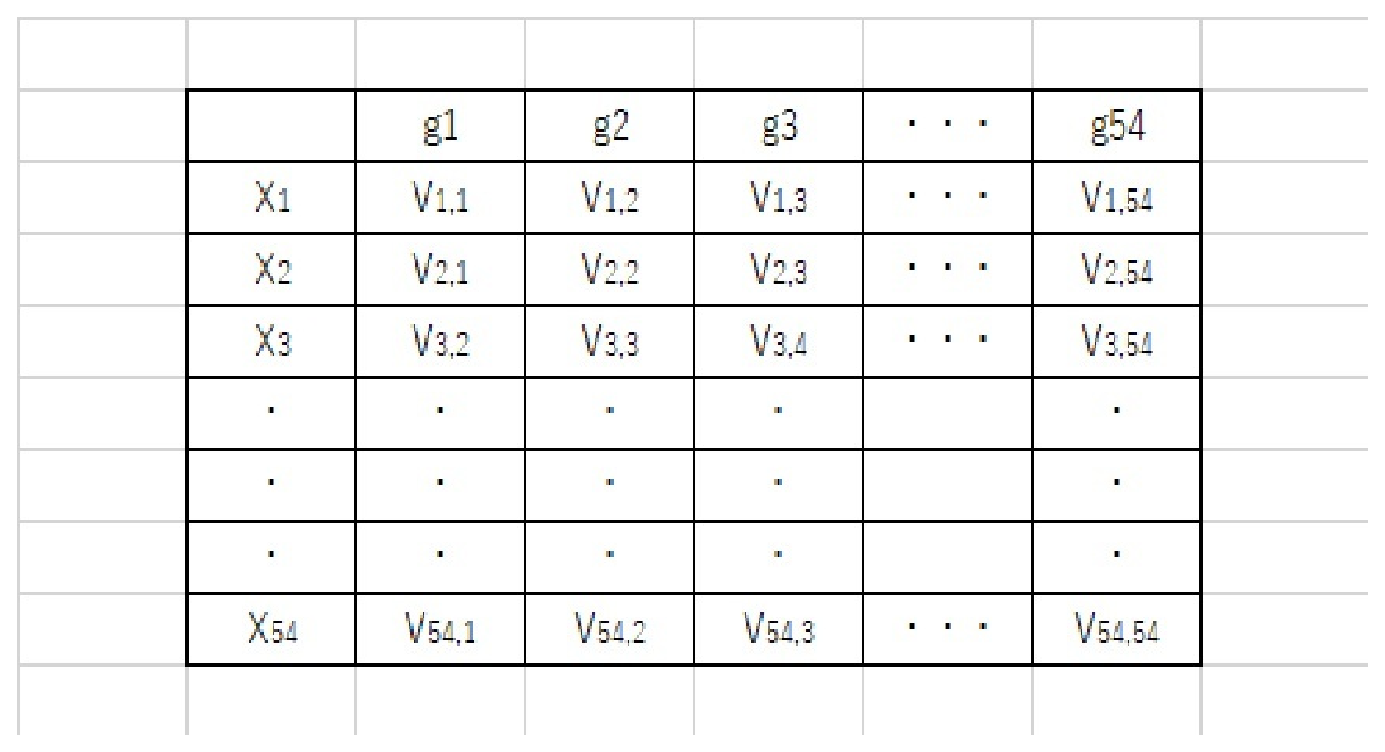
\includegraphics[width=.9\linewidth]{fig/ipusilon0.eps}
  \caption{各制約式の各個体の違反量}
\label{fig:epsilon}
\end{figure}
\begin{figure}[htbp]
  \centering
  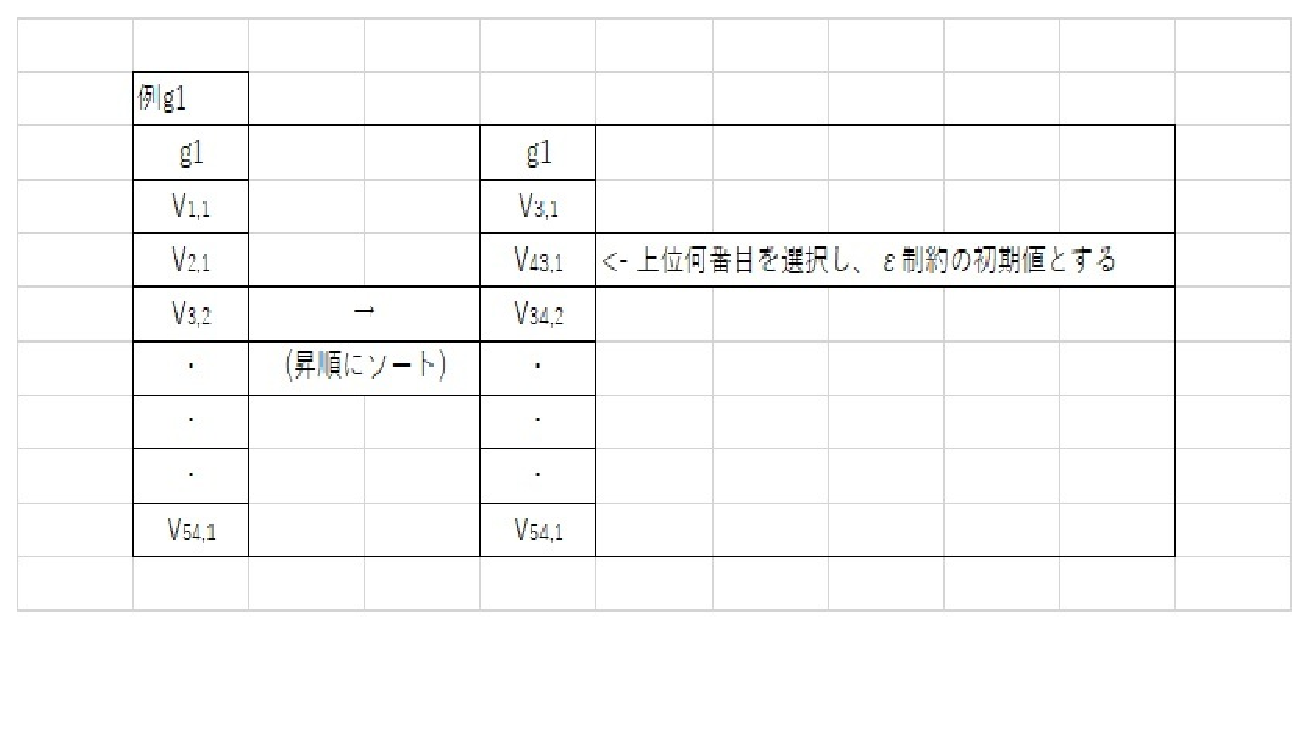
\includegraphics[width=.9\linewidth]{fig/ipusilon1.eps}
  \caption{例:制約g1のε制約}
\label{fig:epsilon1}
\end{figure}



\subsection{ε制約の制御}
探索において、世代が過ぎると同時にε制約を徐々に厳しい条件にし、最後にはε制約を0にすることで、制約違反量を0にするために、ε制約の制御を行う。εレベルを制御する際には、そのレベル以下の個体が常にある程度含まれるようにしながら0まで減少させ、0になった後もある程度の最適化を行うことが望ましいので、$\bm{T}_0(0<{T}_0<{T}_{max})$世代以降は常に0となるよう制御する。よって、以下の世代tのベキ乗関数による制御方法を用い、図\ref{fig:graph1}のように減少させる。
\begin{eqnarray}
\bm{ε}_{t}(m)=
\left\{
\begin{array}{cc}
    \bm{ε}_0(m){(1-\frac{t}{T}_0)}^{cp} & \mbox{$0<t<{T}_0$} \\
    \bm{0} & \mbox{$t\geq{T}_0$}\\
\end{array}
\right.
\end{eqnarray}
$\bm{T}_0$は$\bm{T}_{max}\times{r}(r\in[0,1])$世代とし、cpはベキ乗の係数とする。今回は、個体数50、r=0.9と決めているので、600世代の9割つまり、540世代ごろには全てのε制約を0にするということ。

\begin{figure}[htbp]
  \centering
  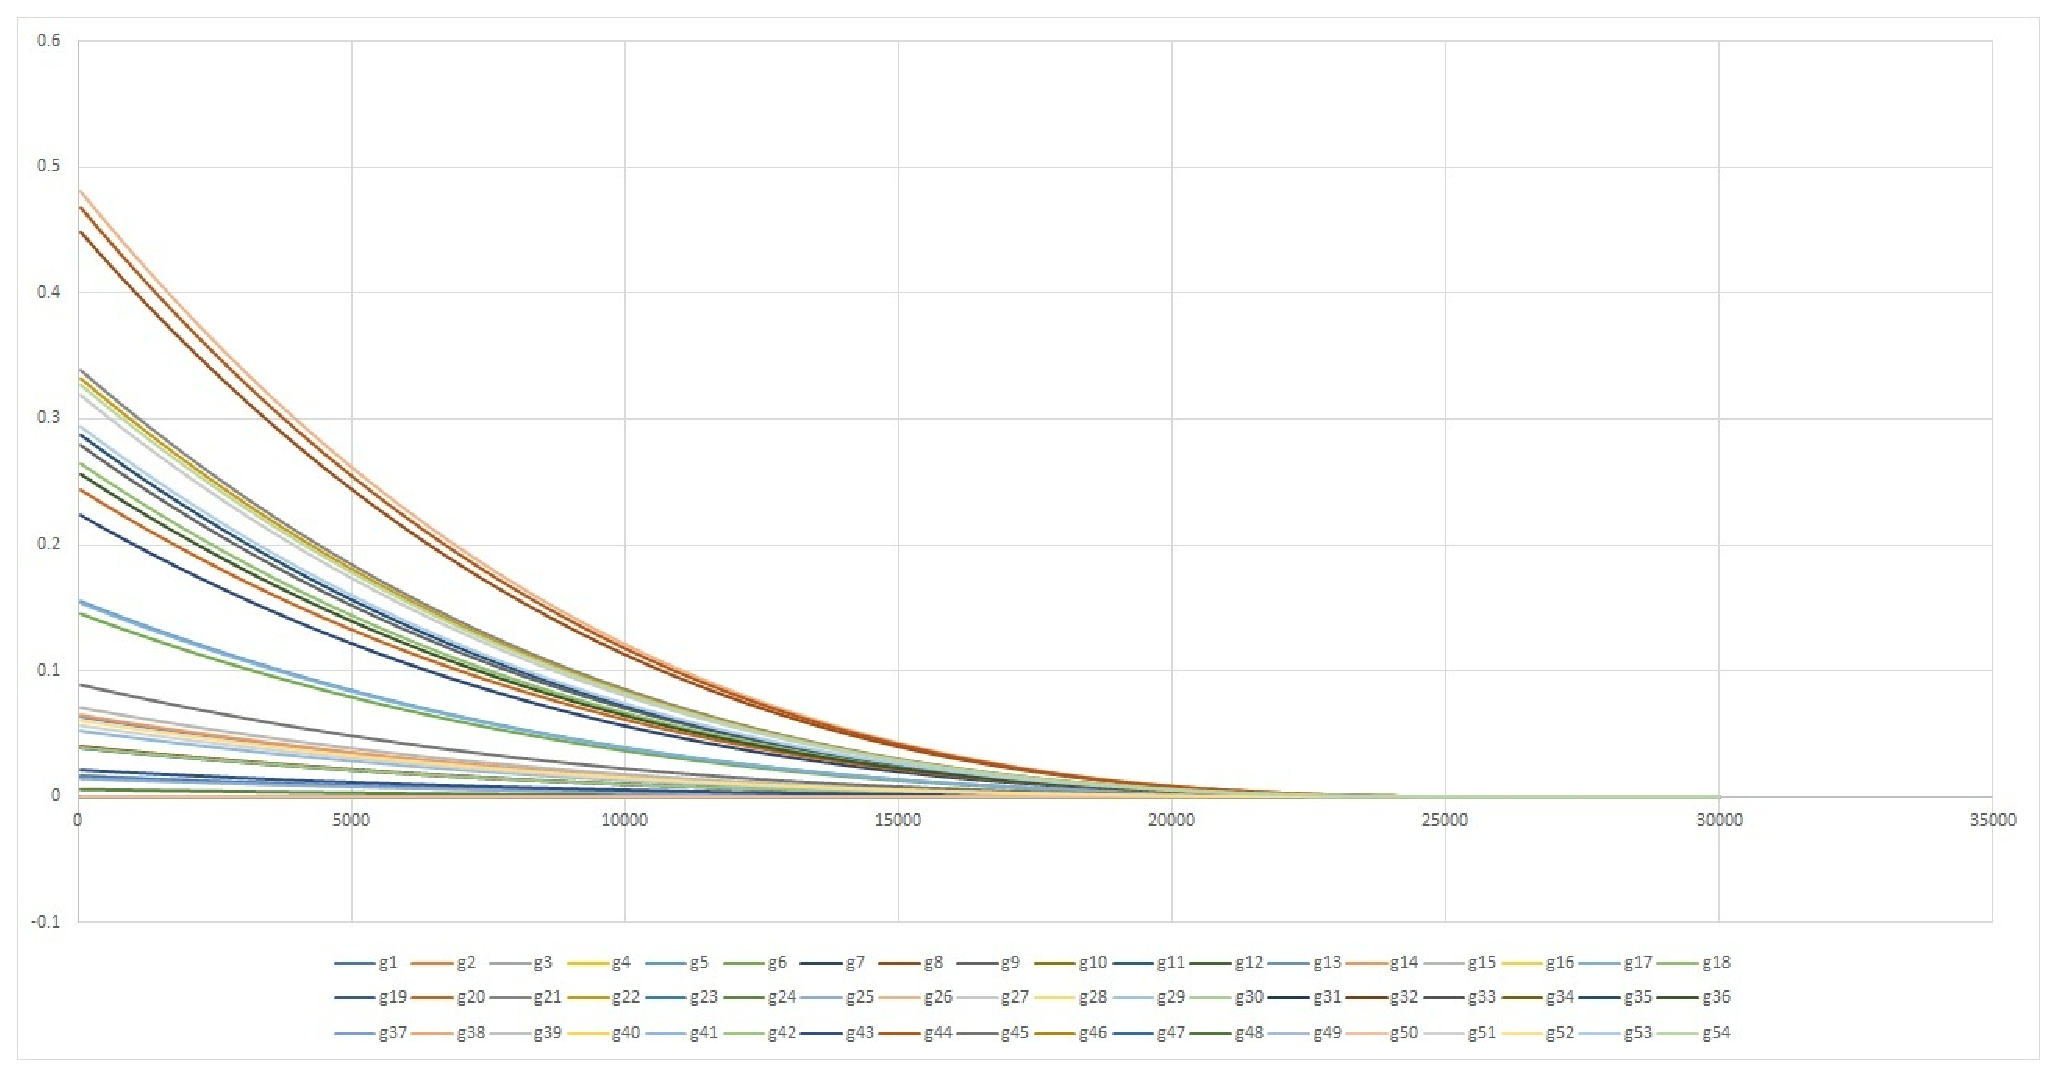
\includegraphics[width=.9\linewidth]{fig/test.eps}
  \caption{各制約ごとのε制約の推移}
  \label{fig:graph1}
\end{figure}

\subsection{制約逸脱度}
ε制約法では、制約をどの程度逸脱しているかを表現するために、制約逸脱度φ(x)を導入する。制約逸脱度φ(x)は、以下を満足する関数である。Fは実行可能状態。
\begin{eqnarray}
\left\{
\begin{array}{cc}
    \bm{φ(x)}=0(x\in{F})\\
    \bm{φ(x)}>0(x\notin{F})\\
\end{array}
\right.
\end{eqnarray}
制約逸脱度関数φ(x)には幾つかの定義方法があるが、今回はG(x)をxの制約逸脱度ベクトルとし、φ(x)は以下のように制約総逸脱度として定義する。
\begin{eqnarray}
%\begin{split}
\bm{G(x)}=(\bm{G}_1(x),\bm{G}_2(x),...,\bm{G}_k(x))\\   
\bm{G}_i(x)=
\left\{
\begin{array}{cc}
     \bm|{g}_i(x)| & \mbox{if${g}_i(x)<0(i=1,2,...,k)$} \\
    \bm{0} & \mbox{otherwise}\\
\end{array}
\right.\\
\bm{φ(x)}=\sum_{i=1}^k \bm{G}_i(x)
%\end{split}
\end{eqnarray}

\subsection{εレベル比較}
目的関数値Fと制約逸脱度φ(x)の改善について、各制約ごとのε制約${ε}_t$を使用し決める。各制約に対する個体ごとに制約違反量g(x)を求め、ε制約と比較し、全ての違反量がε以下の場合は目的関数値の大小関係を優先し、それ以外の場合は制約逸脱度の大小関係を優先する比較であるεレベル比較を定義する。点${x}_1,{x}_2$における関数値を${f}_1,{f}_2$、制約逸脱度を${φ}_1,{φ}_2$とする。定義を以下に示す。
\begin{eqnarray}
\left\{
\begin{array}{cc}
    \bm{f}_1<{f}_2 & \mbox{if${g}_i(x)<{ε}_t(i)(i=1,2,...,54)$}\\
    \bm{f}_1<{f}_2 & \mbox{if${φ}_1={φ}_2$}\\
    \bm{φ}_1<{φ}_2 & \mbox{otherwise}\\
\end{array}
\right.
\end{eqnarray}

\section{ε制約Differential Evolution}
εDEは基本的なアルゴリズムはDEと同様であり、εの制御とεレベル比較を行う点が異なる。今回はεDE/rand/1/binであり、以下にアルゴリズムを示す。
\subsection{初期化}
NP個の初期個体${x}_i$を探索空間S内にランダムに生成し、初期集団P={${x}_i$|i=1,2,...,NP}を構築する。また、各制約ごとのε制約を生成。
\subsection{終了判定}
終了条件を満たせば、アルゴリズムを終了する。
\subsection{突然変異}
各親個体${x}_i$に対して、3個体{$\bm{x}_{r1}$,$\bm{x}_{r2}$,$\bm{x}_{r3}$}を${x}_i$および互いに重複しないように、個体集団Pからランダムに選択する。その後、式\ref{eq:s1}により変異ベクトル${v}_i$を生成する。
\begin{eqnarray}
\bm{v}_i={x}_{r1}+F({x}_{r2}-{x}_{r3})\\
\label{eq:s1}
\end{eqnarray}
ここで、Fは差分の伸縮を表すスケーリングファクタである。
\subsection{交叉}
変異ベクトル${v}_i$を${x}_i$と交叉し、子個体${u}_i$を生成する。交叉はbinomial crossoverを用いる。式を以下で示す。
\begin{eqnarray}
\bm{u}_j=
\left\{
\begin{array}{cc}
    \bm{u}_j & \mbox{if$({rand}_j[0,1]\leq{C}_R \bigvee j={j}_r)$}\\
    \bm{x}_{j,i,g} & \mbox{$otherwise$}\\
\end{array}
\right.
\end{eqnarray}
${rand}_j$は区間[0,1]の一様乱数であり、${j}_i$は[1,D]区間からランダムに選択した変数番号である。また、CRが大きいほど、変異ベクトルの成分が多くuに受け継がれる。

\subsection{生存選択}
子個体を評価し、親個体${x}_i$とεレベル比較を行う。子個体${u}_i$が親個体${x}_i$よりも良ければ子個体が生存者となり、親を子個体で置換する。
\subsection{εレベルの制御}
εレベル制御関数${ε}_t$によって、各制約ごとのεレベルを更新する。
終了判定に戻る。

\section{実験途中結果}
\subsection{実験設定}
目的関数の評価回数の上限は30000回であり、NP=50、最大世代数${T}_{max}$は600世代とした。εレベルの制御のパラメータは、s={0.2,0.5,0.7,0.9}、cp=3とした。また、r=0.9とし、それぞれ1試行の実験を行った。
また、初期値のε制約を各制約の制約違反量から得るようにすると、値が0もしくわ0に近い数値になってしまい、最初から厳しい条件となってしまうので、今回は、各ε制約に対して、各制約ごとの個体の違反数を求め、制約数54で割り、ε制約の初期値にかけて、追加で足している。これは、少しでも最初の条件を緩めるためにしたもので根拠はない。ε制約の初期値の値は今後の課題でもある。
\subsection{実験結果}
r=0.9でパラメータsの値を変化させた結果を表\ref{tbl:MLP1}に示す。

\begin{table}[htbp]
\begin{center}
\caption{F=0.2,CR=0.4,r=0.9,cp=3,s={0.2,0.5,0.7,0.9}}
\label{tbl:MLP1}
\begin{tabular}{|l|c|c|}
\hline
s     & 目的関数値  \\ \hline
s=0.2 & 2.656769\\ \hline
s=0.5 & 2.647150\\ \hline
s=0.7 & 2.652573\\ \hline
s=0.9 & 2.628328\\ \hline
\end{tabular}
\end{center}
\end{table}
また、上記のパラメータごとに目的関数値と制約逸脱度をグラフにしたものを図\ref{fig:graph4}、図\ref{fig:graph5}、図\ref{fig:graph6}、図\ref{fig:graph7}、に示す。なお、青色の線は目的関数値の推移で、橙色の線は制約逸脱度の推移である。
\begin{figure}[htbp]
  \centering
  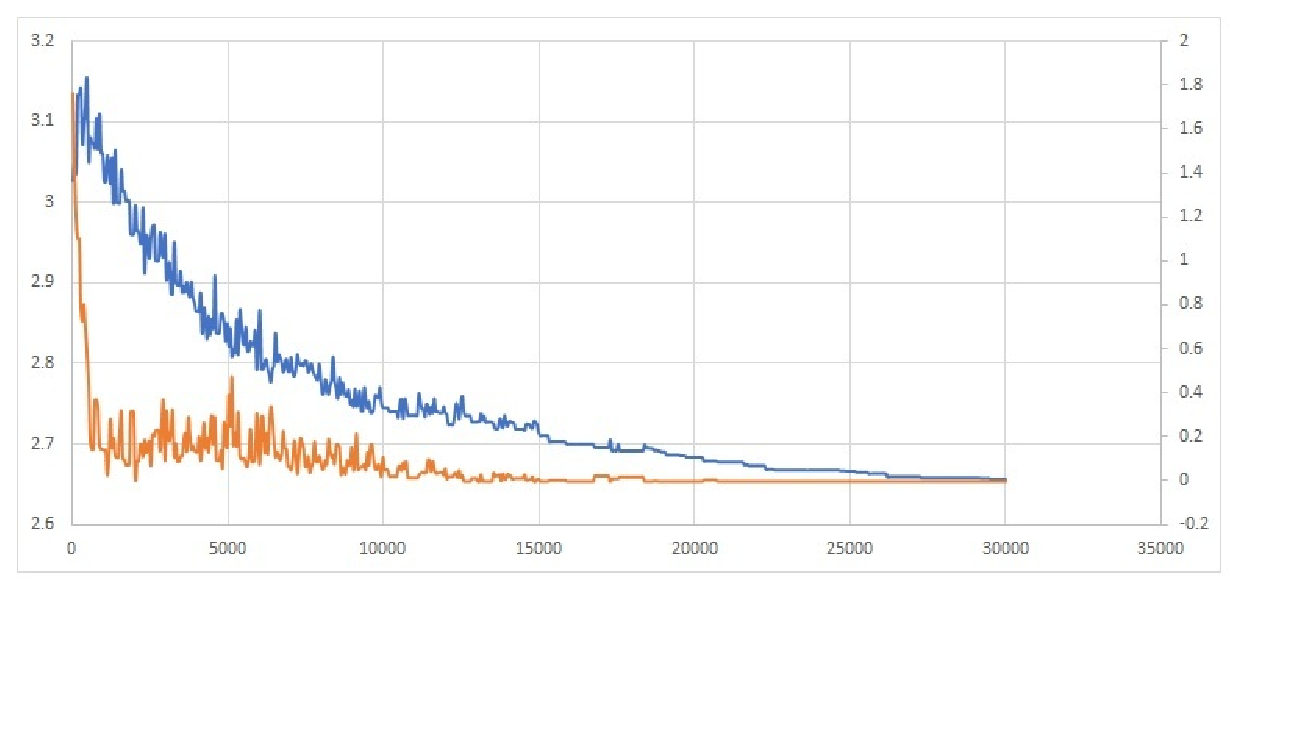
\includegraphics[width=.9\linewidth]{fig/s=0.2.eps}
  \caption{s=0.2}
\label{fig:graph4}
\end{figure}
\begin{figure}[htbp]
  \centering
  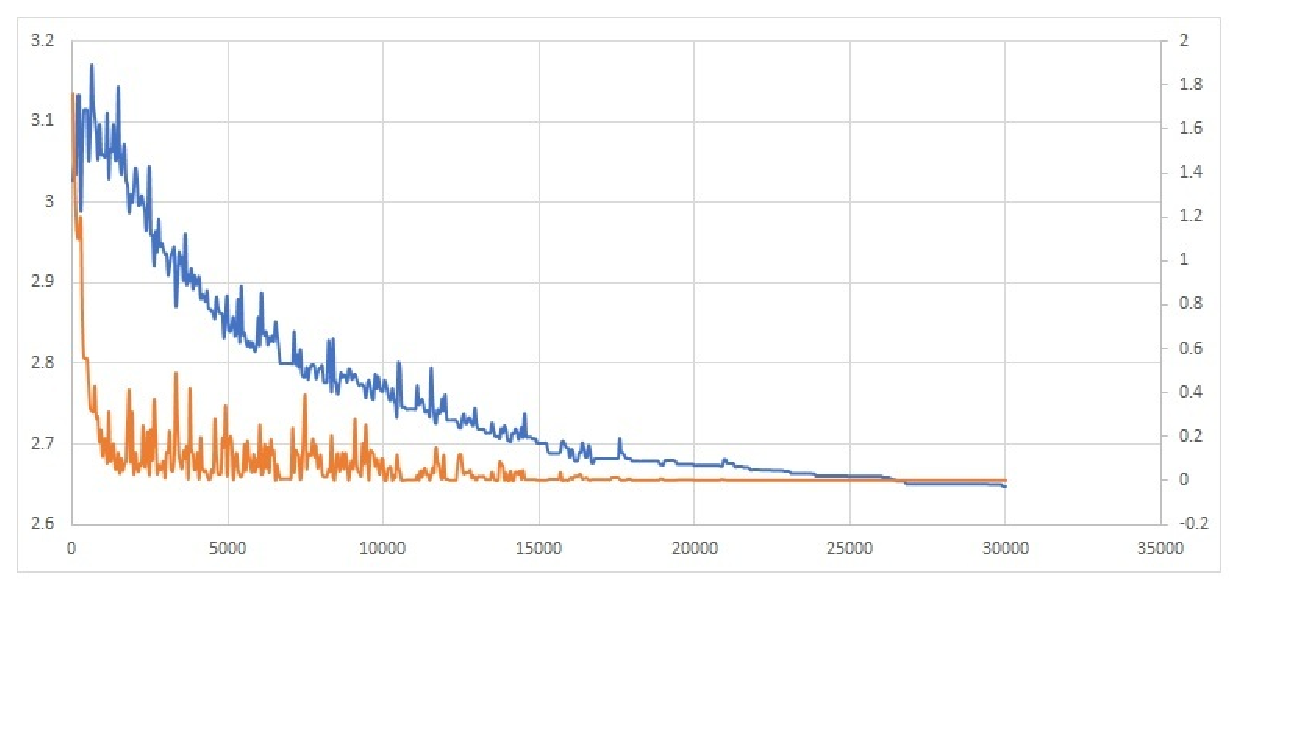
\includegraphics[width=.9\linewidth]{fig/s=0.5.eps}
  \caption{s=0.5}
\label{fig:graph5}
\end{figure}
\begin{figure}[htbp]
  \centering
  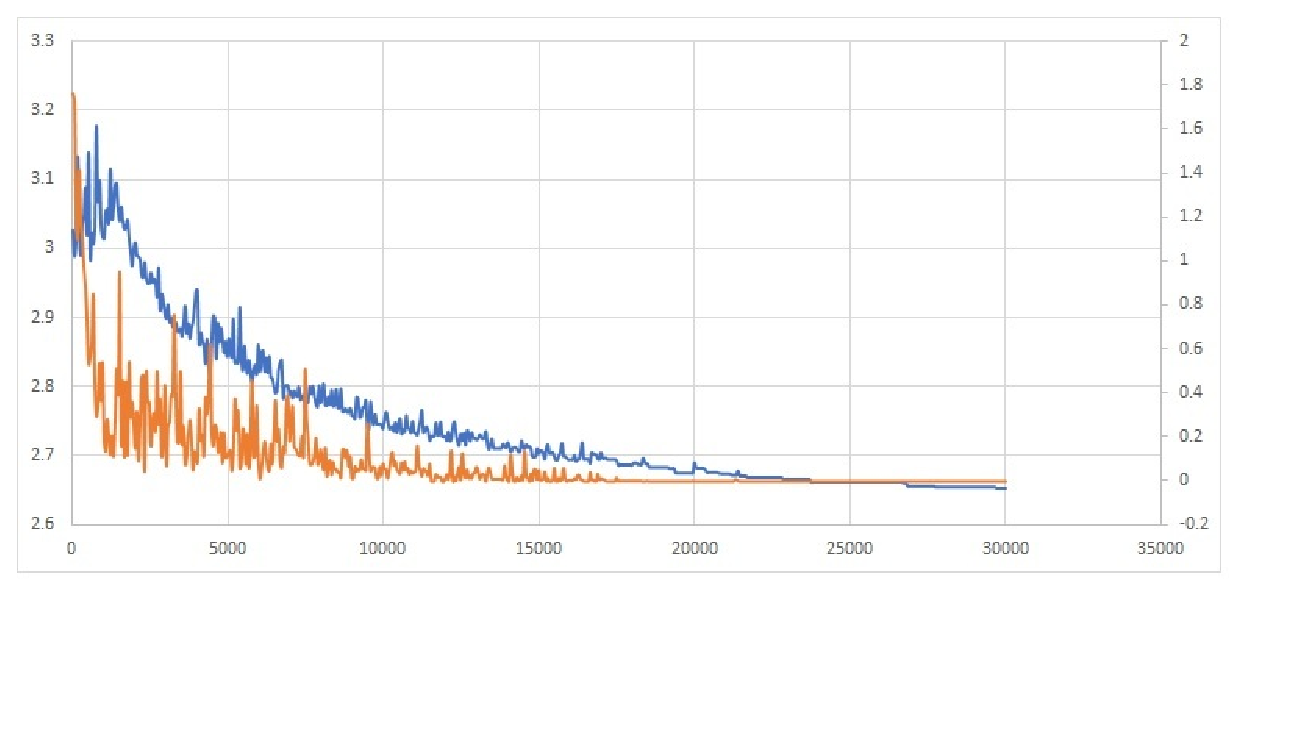
\includegraphics[width=.9\linewidth]{fig/s=0.7.eps}
  \caption{s=0.7}
\label{fig:graph6}
\end{figure}
\begin{figure}[htbp]
  \centering
  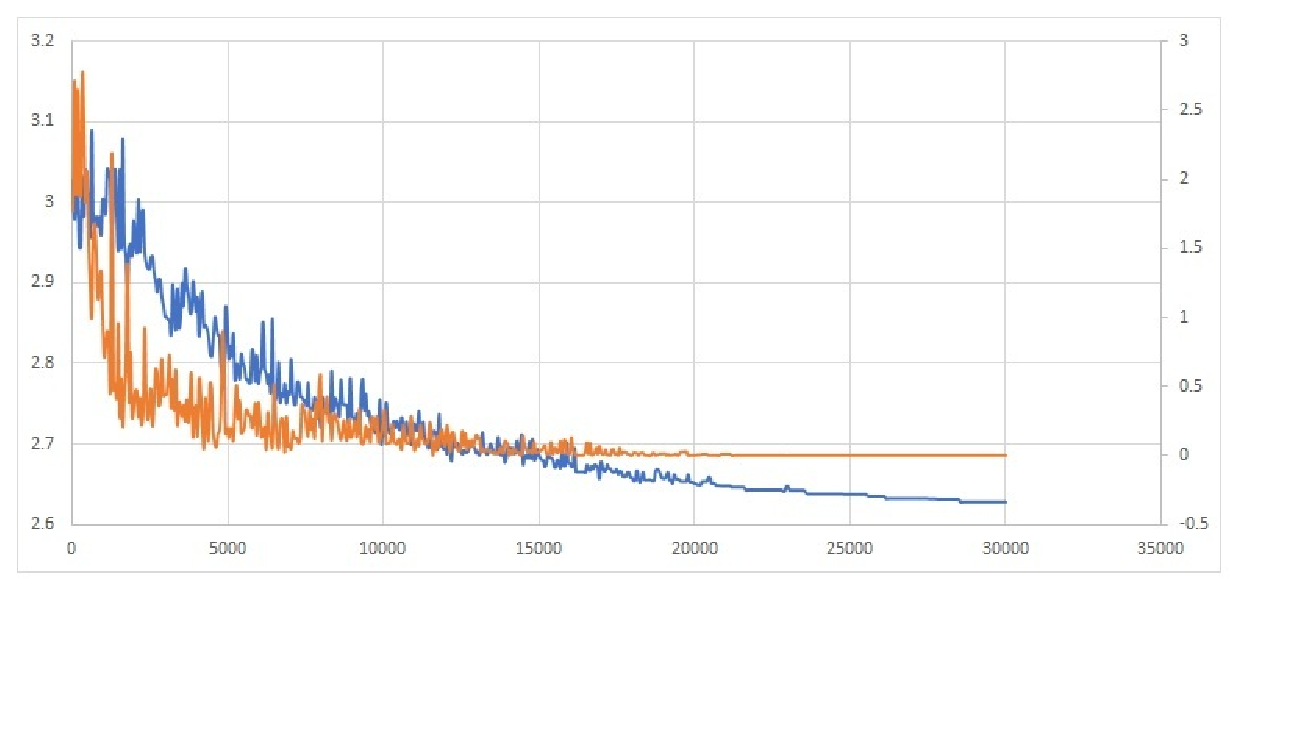
\includegraphics[width=.9\linewidth]{fig/s=0.9.eps}
  \caption{s=0.9}
\label{fig:graph7}
\end{figure}

F=0.2,CR=0.4,cp=3,r=0.9のパラメータは今まで実験した中で一番良い結果になったので、そうしています。

sのパラメータは、1に近いほうが、少しではあるがε制約の初期値を高い値にして、条件を緩めてくれる。これにより、s=0.9のパラメータでは、図\ref{fig:graph7}を見る通り、制約逸脱度が他のパラメータの時より緩やかに減少しているのが分かる。そのため、目的関数値もそこまで最初の時点で改悪されていない。しかし、このやり方では、まだ制約逸脱度が先に改善され、目的関数値をバランスよく改善できてなく、最適値もまだ高いので課題である。

\section{今後の課題}
・目的関数値と制約逸脱度の分布のバランスよくするために、工夫する。
・一つ一つのε制約の値が小さすぎて条件が厳しすぎる。
(新しい手法)
・個体ごとにε制約をもつようにする。
・各制約ごとのε制約を、世代ごとで、一番違反量の高い制約のε制約を使うようにする。

\bibliography{btxsample}
\bibliographystyle{jplain}

%欧文用	和文用	特徴
%plain	jplain	参考文献をアルファベット順で出力する
%unsrt	junsrt	参考文献を引用された順で出力する

\section{参考文献}
[1]ε制約法とパレート的アプローチを用いたDifferential Evolutionによる複数車種車両の同時最適化 著者:串田淳一、原章、高濱徹行 出版:進化計算学会論文誌 URL:https://ci.nii.ac.jp/naid/130007797834\\

[2]難易度による制約分割を用いた段階的制約充足法の適用に関する検討著者:丹羽健斗、古川大弘 出版:第14回進化計算学会研究会 URL:https://kaken.nii.ac.jp/grant/KAKENHI-PROJECT-15K00336/






\end{document}